%!TEX root = ../thesis.tex

\section{実験1}
\subsection{実験目的}
シミュレータ上で実験を行い, 提案手法の有効性を検証する.

\subsection{実験装置}
実験は, \figref{Fig:gazebo}に示すGazebo\cite{gazebo}のWillow Garage\cite{willow}で\figref{Fig:willow-garage}に示すコースで一周行う. また, ロボットモデルには\figref{Fig:turtlebot3}に示すようなカメラを3つ搭載したTurtlebot3\cite{turtlebot3}を用いた. 

\begin{figure}[h]
  \centering
  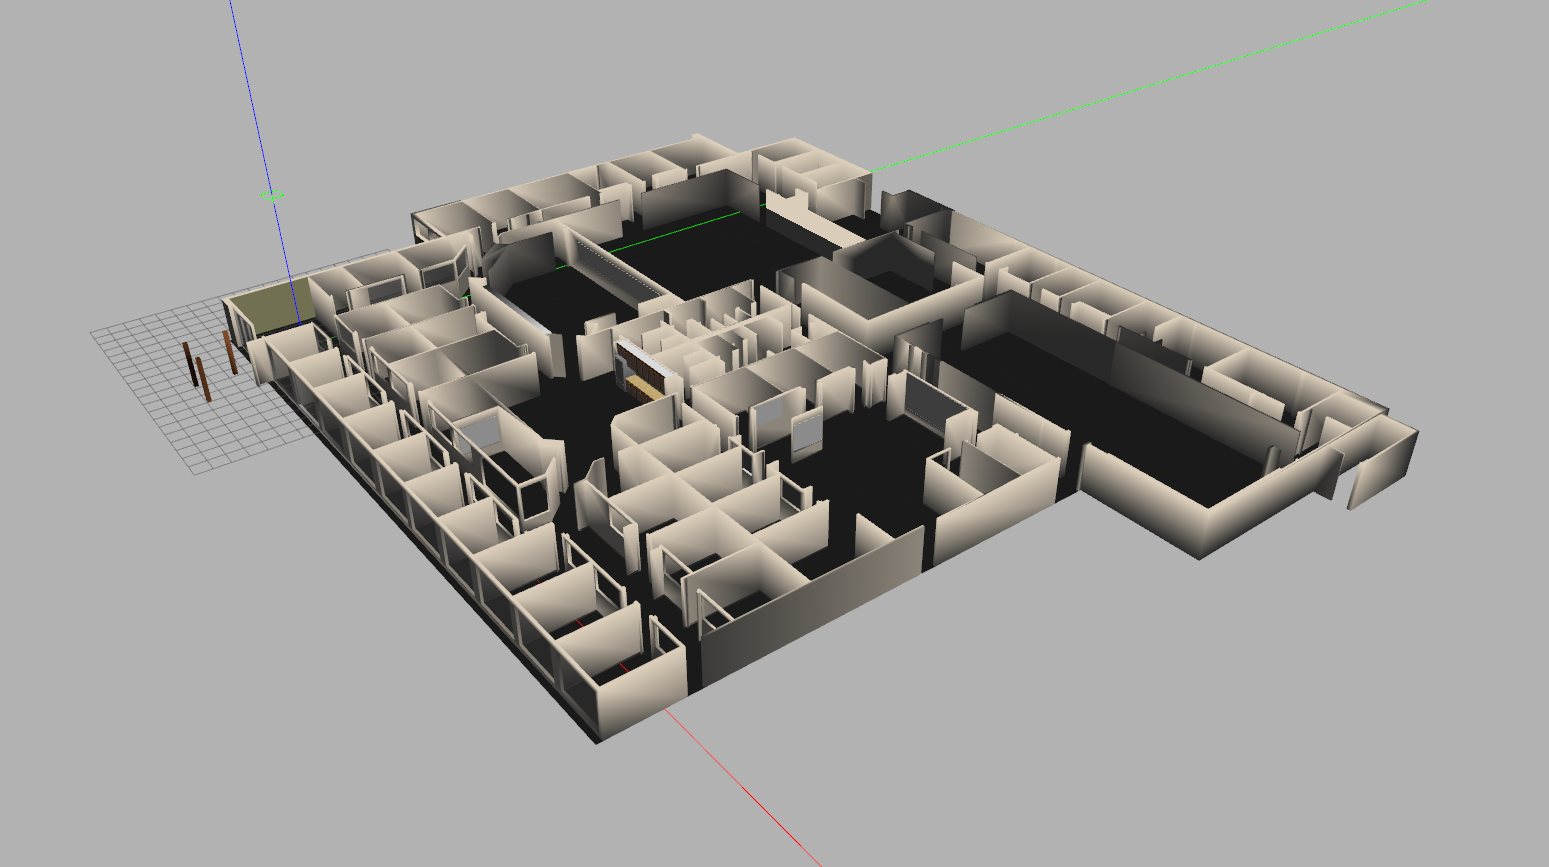
\includegraphics[keepaspectratio, scale=0.15]{images/gazebo.png}
  \caption{Experimental environment in simulator}
  \label{Fig:gazebo}
  \end{figure}

\begin{figure}[h]
  \centering
  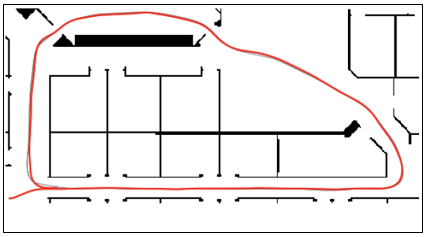
\includegraphics[keepaspectratio, scale=0.5]{images/willow-garage.png}
  \caption{Course to collect data}
  \label{Fig:willow-garage}
  \end{figure}

\begin{figure}[h]
  \centering
  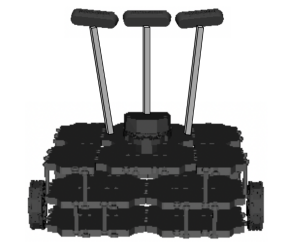
\includegraphics[keepaspectratio, scale=0.55]{images/turtlebot3.png}
  \caption{Turtlebot3 waffle with 3 cameras}
  \label{Fig:turtlebot3}
  \end{figure}

\newpage
\subsection{実験方法}
\begin{description}
  \item[1.データ収集フェーズ]データの収集方法について述べる. \figref{Fig:old-method}にデータの収集方法を示す. 赤色の線である目標経路から平行に±0.10, ±0.20, ±0.30m離れた座標にロボットを配置する. そして, その座標ごとに目標経路に沿った向きを基準として±5度傾けて, カメラ画像とナビゲーションの出力である角速度を収集する. これを\figref{Fig:willow-garage}に示した経路で実験を行う. 
\end{description}

\begin{figure}[h]
  \centering
  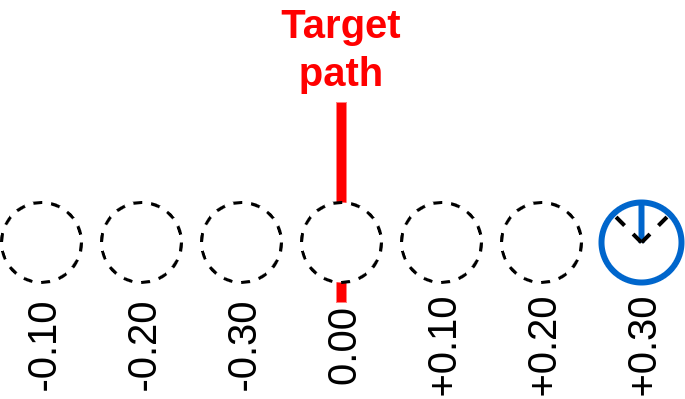
\includegraphics[keepaspectratio, scale=0.25]{images/old-method.png}
  \caption{Method of collecting data around the target route}
  \label{Fig:old-method}
  \end{figure}

\newpage
\begin{description}
  \item[2.訓練フェーズ] データ量2658, 先行研究に倣ってバッチ数8, 実験1では4000step, 実験2では8000step, 実験3では10000step学習した. なお, 4000stepは従来研究において, シミュレータの実験に用いられてきたステップ数であり, 10000stepは従来研究において, 実ロボットの実験に用いられていたステップ数である. 
\end{description}

\begin{description}
  \item[3.テストフェーズ]\figref{Fig:willow-garage}に示すコースで, 10回走行させる. 壁に衝突せずに一周できた場合を成功とし, 壁に激突したり, コースアウトして経路に復帰できなかった場合を失敗とした.
\end{description}

\subsection{実験結果}
実験結果を表\ref{tb:exp1}に示す. また, 失敗箇所は\figref{Fig:result1}, 実験ごとの失敗箇所における失敗回数は\ref{tb:fail1}のようになった. 

\begin{table}[h]
  \centering
  \begin{tabular}{|c|c|} \hline
    Experiments & Number of successes \\ \hline
    Exp.1(4000step) & 0/10 \\ \hline
    Exp.2(8000step) & 0/10 \\ \hline
    Exp.3(10000step) & 0/10 \\ \hline
  \end{tabular}
  \caption{Number of successes in the experiment1}
  \label{tb:exp1}
\end{table}

\begin{figure}[h]
  \centering
  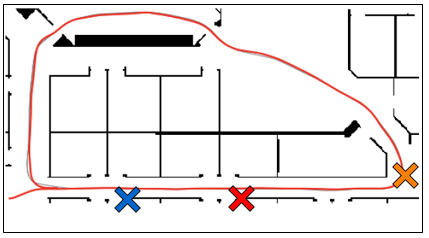
\includegraphics[keepaspectratio, scale=0.5]{images/result1.png}
  \caption{Failure point of the experiment}
  \label{Fig:result1}
  \end{figure}

\begin{table}[h]
  \centering
  \begin{tabular}{|c|c|c|} \hline
    Experiments & Number of failures with red x & Number of failures with blue x \\ \hline
    Exp.1(4000step) & 1 & 9 \\ \hline
    Exp.2(8000step) & 0 & 10 \\ \hline
    Exp.3(10000step) & 0 & 10 \\ \hline
  \end{tabular}
  \caption{Number of failures in the experiment}
  \label{tb:fail1}
\end{table}

\newpage
\subsection{考察}
ステップ数を増やしても成功回数は増えなかった.  また, 目標経路から離れた際に戻る挙動や, 壁に近づきすぎた際に避ける挙動も見られなかった. ここで, 訓練させた際の各実験ごとのlossを\figref{Fig:exp1-4000}, \figref{Fig:exp1-8000}, \figref{Fig:exp1-10000}に示す. 実験1から実験3全てにおいて, オーバーシュートしていると考えられる. そこで, 収集した角速度を\figref{Fig:exp1}のようにヒストグラムにした. これより, 経路上及び経路周辺のデータである0rad/sから0.1rad/sが全体の4割程度しかないことが分かる. 以上を踏まえて, 経路上及び経路周辺のデータが多い方が, 経路追従の成功回数が増えるのではないかと考えた. 

\newpage
\begin{figure}[h]
  \centering
  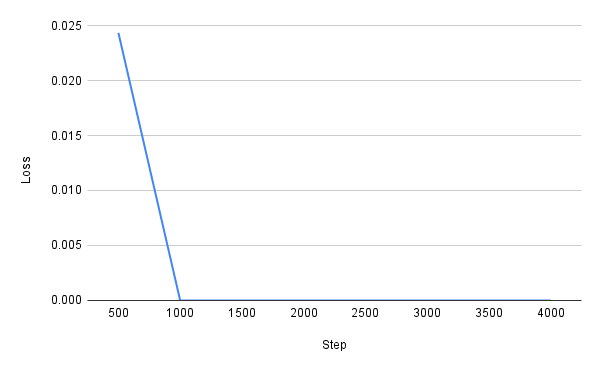
\includegraphics[keepaspectratio, scale=0.31]{images/exp1-4000.png}
  \caption{Loss value in the experiment1}
  \label{Fig:exp1-4000}
  \end{figure}

\begin{figure}[h]
  \centering
  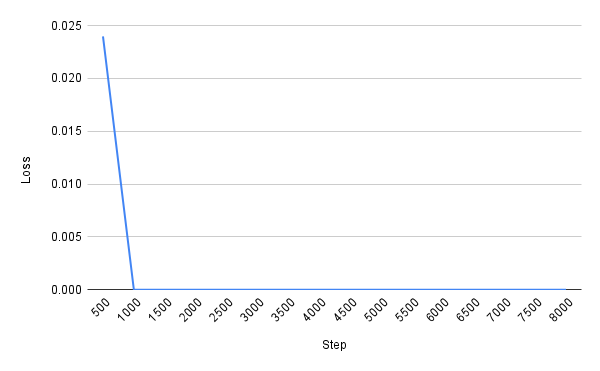
\includegraphics[keepaspectratio, scale=0.31]{images/exp1-8000.png}
  \caption{Loss value in the experiment2}
  \label{Fig:exp1-8000}
  \end{figure}

\begin{figure}[h]
  \centering
  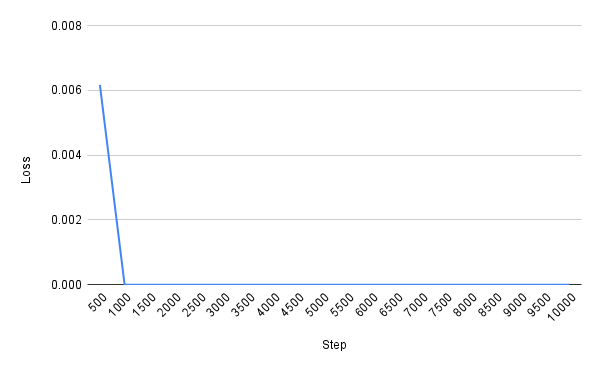
\includegraphics[keepaspectratio, scale=0.31]{images/exp1-10000.png}
  \caption{Loss value in the experiment3}
  \label{Fig:exp1-10000}
  \end{figure}

\begin{figure}[h]
  \centering
  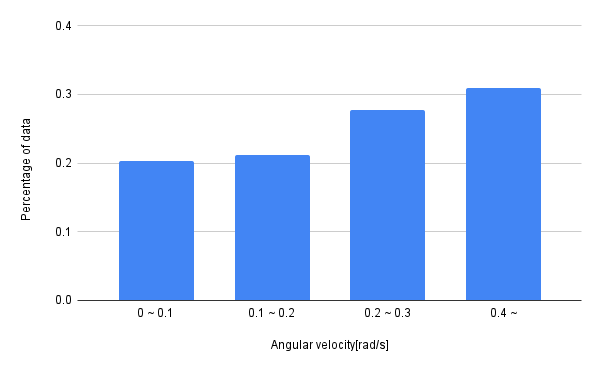
\includegraphics[keepaspectratio, scale=0.4]{images/exp1.png}
  \caption{Histogram of collected angular velocities in the experiment1}
  \label{Fig:exp1}
  \end{figure}

\newpage
\section{実験2}
実験目的, 実験装置, テストフェーズは実験条件1と同様である.
\subsection{実験方法}
\begin{description}
  \item[1.データ収集フェーズ]実験1を踏まえて, 経路周辺のデータを多く取得する手法を試みる. \figref{Fig:collect-data}にデータの収集方法を示す. 赤色の線である目標経路から平行に±0.01, ±0.02, ±0.04, ±0.06, ±0.08, ±0.10, ±0.15, ±0.20, ±0.30m離れた座標にロボットを配置する. そして, 手法1と同様にロボットを傾けて画像と角速度を\figref{Fig:collect-data2}のように収集する. これを\figref{Fig:willow-garage}に示すコースで一周行う.  
\end{description}

\begin{figure}[h]
  \centering
  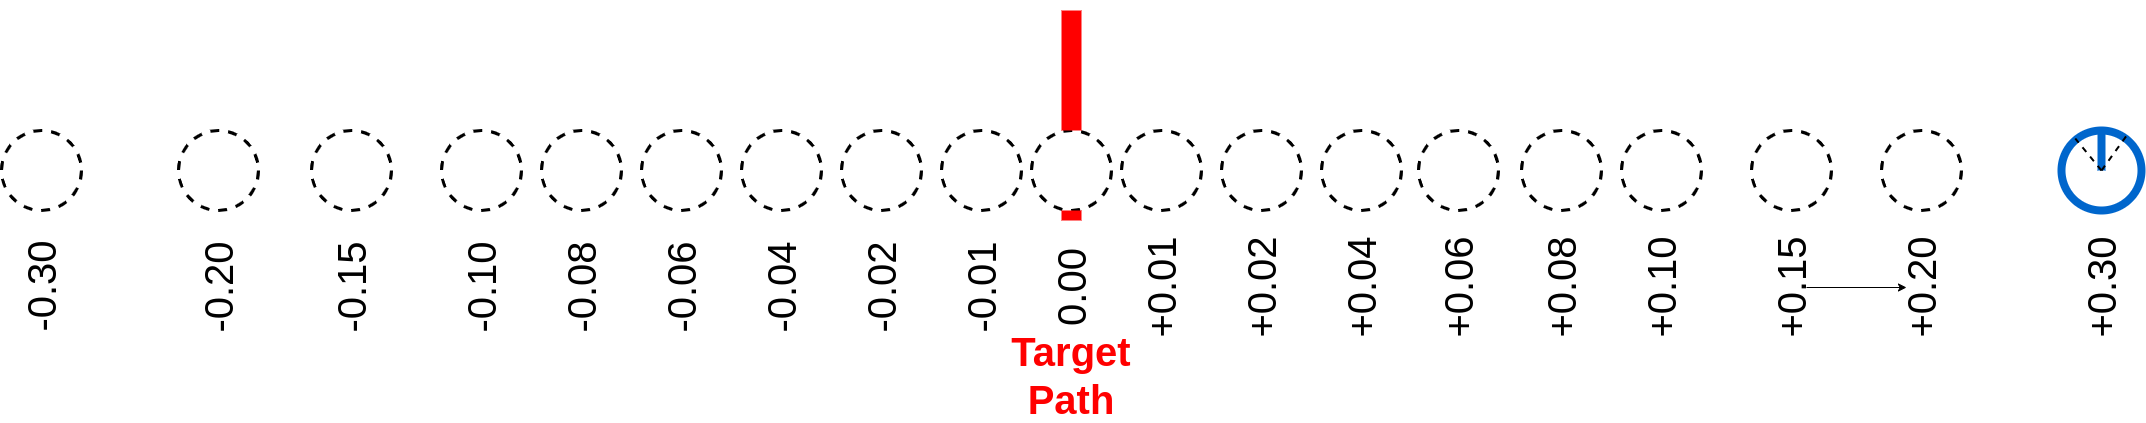
\includegraphics[keepaspectratio, scale=0.18]{images/collect-data.png}
  \caption{Method of collecting data around the target route}
  \label{Fig:collect-data}
  \end{figure}

\begin{description}
  \item[2.訓練フェーズ]データ量7242, バッチ数8, ステップ数は実験条件1と同様に4000step, 8000step, 10000step学習した. 
\end{description}

\subsection{実験結果}
実験結果を表\ref{tb:exp2}に示す. また, 失敗箇所は\figref{Fig:result2}, 実験ごとの失敗箇所における失敗回数は\ref{tb:fail2}であった. 

\begin{table}[h]
  \centering
  \begin{tabular}{|c|c|} \hline
    Experiments & Number of successes \\ \hline
    Exp.1(4000step) & 0/10 \\ \hline
    Exp.2(8000step) & 0/10 \\ \hline
    Exp.3(10000step) & 0/10 \\ \hline
  \end{tabular}
  \caption{Number of successes in the experiment}
  \label{tb:exp2}
\end{table}

\begin{figure}[h]
  \centering
  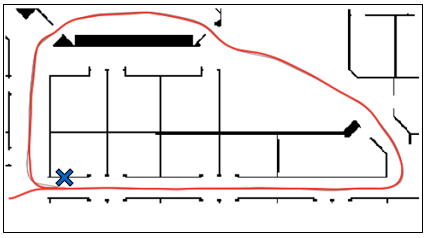
\includegraphics[keepaspectratio, scale=0.5]{images/result2.png}
  \caption{Failure point of the experiment2-1}
  \label{Fig:result2}
  \end{figure}

\begin{table}[h]
  \centering
  \begin{tabular}{|c|c|c|} \hline
    Experiments & Number of failures with blue x \\ \hline
    Exp.1(4000step) & 10 \\ \hline
    Exp.2(8000step) & 10 \\ \hline
    Exp.3(10000step) & 10 \\ \hline
  \end{tabular}
  \caption{Number of failures in the experiment}
  \label{tb:fail2}
\end{table}

\newpage
\paragraph{考察}
収集した角速度を\figref{Fig:exp2}のようにヒストグラムにした. 経路上及び経路周辺のデータが\figref{Fig:exp1}と比べて多くなっている. これにより, \figref{Fig:result2}の青枠の区間において, 壁に衝突することなく走行できていることが分かる. しかし, 経路上や経路周辺のデータを増やしたり, ステップ数を増やしたりしても成功回数は増えなかった. ここで, 訓練させた際の各実験ごとのlossを\figref{Fig:exp2-4000}, \figref{Fig:exp2-8000}, \figref{Fig:exp2-10000}に示す. 実験条件1と同様に実験1から実験3全てにおいて, オーバーシュートしていると考えられる. そこで, 先行研究のオンライン学習では計算のリソースなどの観点からバッチ数を8にしていたが, 提案手法ではオフラインで学習を行うため, バッチ学習に変更する. これにより, 一度に大量のデータを扱えるため最適解に辿り着くことができ, 成功回数が増えるのではないかと考えた. 

\begin{figure}[h]
  \centering
  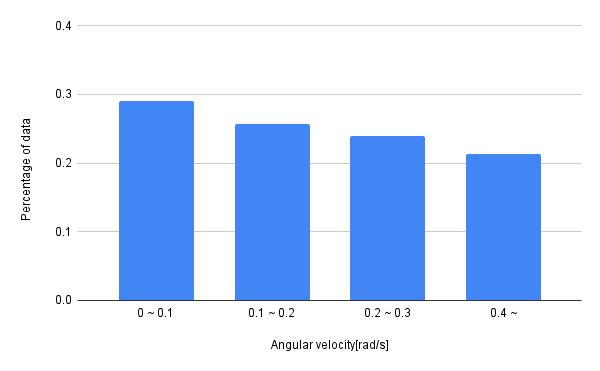
\includegraphics[keepaspectratio, scale=0.4]{images/exp2.png}
  \caption{Histogram of collected angular velocities in the experiment2-1}
  \label{Fig:exp2}
  \end{figure}

\newpage
\begin{figure}[h]
  \centering
  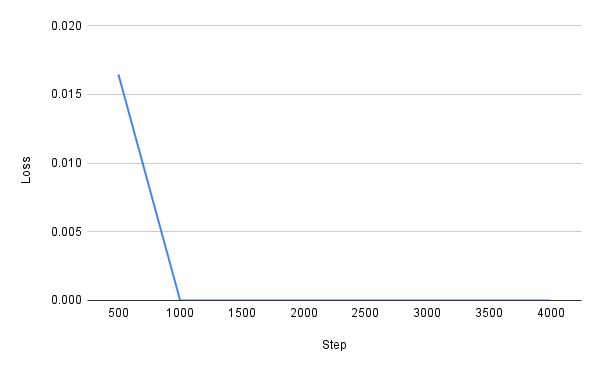
\includegraphics[keepaspectratio, scale=0.31]{images/exp2-4000.png}
  \caption{Loss value in the experiment1}
  \label{Fig:exp2-4000}
  \end{figure}

\begin{figure}[h]
  \centering
  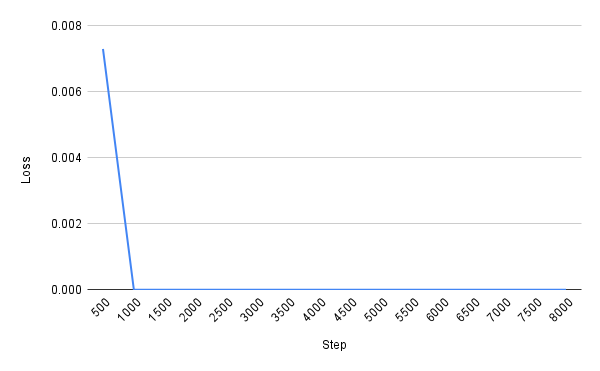
\includegraphics[keepaspectratio, scale=0.31]{images/exp2-8000.png}
  \caption{Loss value in the experiment2}
  \label{Fig:exp2-8000}
  \end{figure}

\begin{figure}[h]
  \centering
  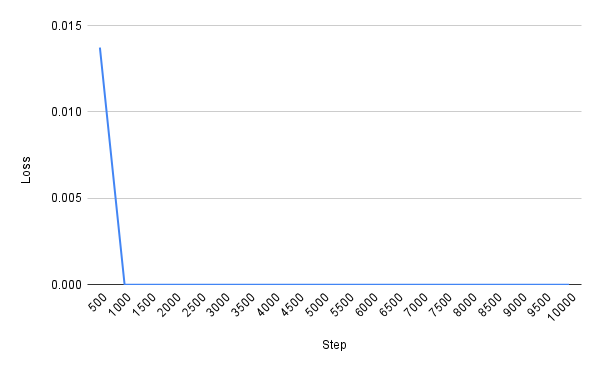
\includegraphics[keepaspectratio, scale=0.31]{images/exp2-10000.png}
  \caption{Loss value in the experiment3}
  \label{Fig:exp2-10000}
  \end{figure}
  
\newpage
\section{実験3}
オフラインで学習を行うメリットを活かして, ここではバッチ学習を用いることで成功回数が増えるか検証する. 実験目的, 実験装置, データ収集フェーズは実験2と同様である. 

\begin{description}
  \item[2.訓練フェーズ] バッチサイズはデータ量と同じ7242, バッチ学習で実験条件1, 2と同様に4000step, 8000step, 10000step学習した. 
\end{description}

\subsection{実験結果}
実験結果を\ref{tb:exp3}に示す. また, 失敗箇所\figref{Fig:result3}, 実験ごとの失敗箇所における失敗回数は\ref{tb:fail3}のようになった.

\begin{table}[h]
  \centering
  \begin{tabular}{|c|c|} \hline
    Experiments & Number of successes \\ \hline
    Exp.1(4000step) & 0/10 \\ \hline
    Exp.2(8000step) & 1/10 \\ \hline
    Exp.3(10000step) & 1/10 \\ \hline
  \end{tabular}
  \caption{Number of successes in the experiment2-2}
  \label{tb:exp3}
\end{table}

\begin{figure}[h]
  \centering
  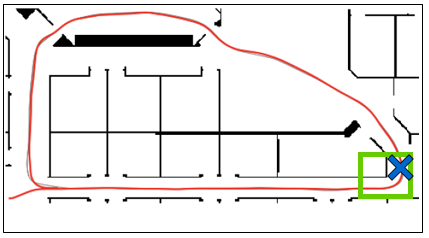
\includegraphics[keepaspectratio, scale=0.6]{images/result3.png}
  \caption{Failure point of the experiment2-2}
  \label{Fig:result3}
  \end{figure}

\begin{table}[h]
  \centering
  \begin{tabular}{|c|c|c|} \hline
    Experiments & Number of failures with blue x \\ \hline
    Exp.1(4000step) & 10 \\ \hline
    Exp.2(8000step) & 9 \\ \hline
    Exp.3(10000step) & 9 \\ \hline
  \end{tabular}
  \caption{Number of failures in the experiment}
  \label{tb:fail3}
\end{table}

\paragraph{考察}
4000stepでは成功回数が0/10だったが, 8000step, 10000stepにすることで成功回数が1/10になり, 目標経路を一周することができた. このことから, 訓練する際に異常データから受ける影響が少なくて済むバッチ学習を用いて, ステップ数を増やすことで成功回数が増えることを示せた. また, lossは\figref{Fig:exp3-4000}, \figref{Fig:exp3-8000}, \figref{Fig:exp3-10000}のようになった. 失敗箇所は\figref{Fig:result3}の緑枠内の角で4000step, 8000step, 10000step全てで曲がりきれず, 青×に示す箇所でコースアウトした. しかし, 実験条件2と比べて角で曲がる挙動が見られた. 以上から, 成功回数は増えたが, 実験条件3では成功回数が十分であるとは言えず, ほとんどで角を曲がり切れていない. そこで, \figref{Fig:result3}の緑枠内のデータを増やすことで角を曲がり切ることができ, 成功回数が増えるのではないかと考えた. 

\newpage
\begin{figure}[h]
  \centering
  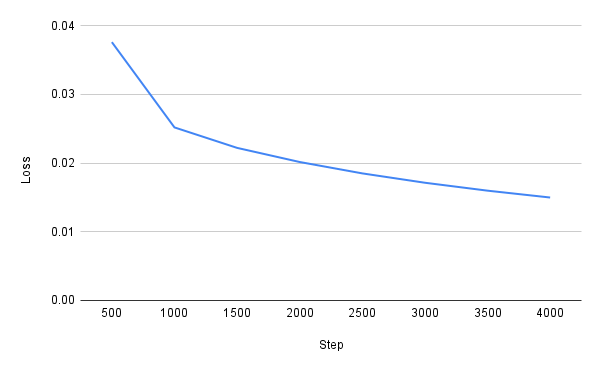
\includegraphics[keepaspectratio, scale=0.31]{images/exp3-4000.png}
  \caption{Loss value in the experiment1}
  \label{Fig:exp3-4000}
  \end{figure}

\begin{figure}[h]
  \centering
  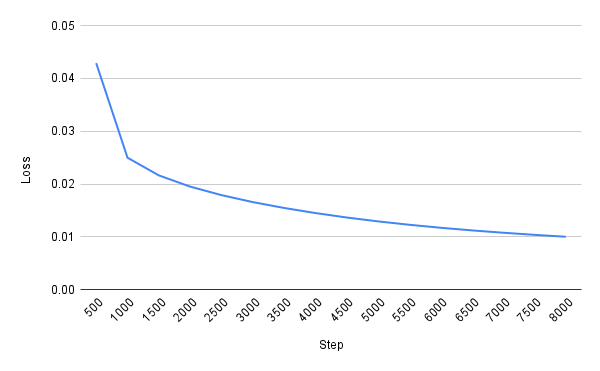
\includegraphics[keepaspectratio, scale=0.31]{images/exp3-8000.png}
  \caption{Loss value in the experiment2}
  \label{Fig:exp3-8000}
  \end{figure}

\begin{figure}[h]
  \centering
  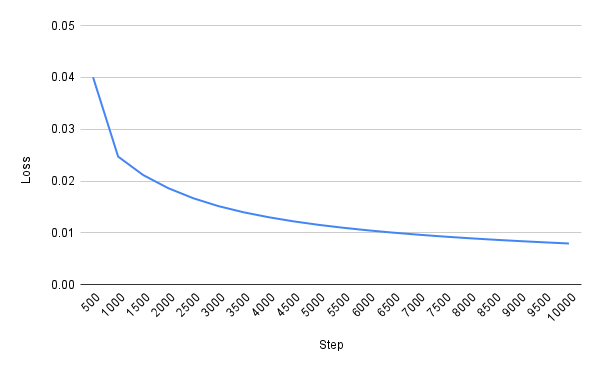
\includegraphics[keepaspectratio, scale=0.31]{images/exp3-10000.png}
  \caption{Loss value in the experiment3}
  \label{Fig:exp3-10000}
  \end{figure}

\newpage

\section{実験4}
ここでは, 角のデータを増やすことで成功回数が増えるかどうか検証する. 実験条件3で用いた角速度のデータを\figref{Fig:exp3}に示す. 直進に近いデータ(-0.2rad/sから0.2rad/s)の合計は4227, 角を左折する際の角速度のデータ(0.3rad/s以上)の合計は1280である. 直進は失敗していないことから, 左折する際のデータも直進と同量であれば曲がれるのではないかと考えた. よって, 左折する際のデータ量を4倍して実験を行う. 

\begin{figure}[h]
  \centering
  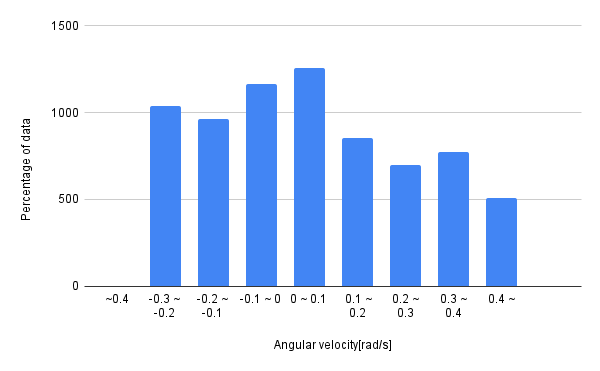
\includegraphics[keepaspectratio, scale=0.4]{images/exp3.png}
  \caption{Histogram of collected angular velocities in the experimental condition 3}
  \label{Fig:exp3}
  \end{figure}

\paragraph{データ収集フェーズ}
データの収集方法は, 目標経路に対して平行な方向は実験2, 3と同様であるが, 実験条件4では目標経路に沿った向きのロボットの配置間隔を変更する. 実験条件1から実験条件3では目標経路に沿った向きで0.5m間隔でロボットを配置していた. しかし, 実験条件3の\figref{Fig:result3}でも示したように, 緑枠内において目標経路に沿った向きのロボットの配置間隔を0.25mに変更する. これにより, 角においてのデータ量が増えるため, 角を曲がることができ, 成功回数が増えることが期待できる. 

\paragraph{訓練フェーズ}
バッチサイズはデータ量と同じ?個, バッチ学習で4000step, 8000stp, 10000step学習した. 

\subsection{実験結果}
実験結果は, \ref{tb:exp4}のようになった. 

\begin{table}[h]
  \centering
  \begin{tabular}{|c|c|} \hline
    Experiments & Number of successes \\ \hline
    Exp.1(4000step) & /10 \\ \hline
    Exp.1(8000step) & /10 \\ \hline
    Exp.1(10000step) & /10 \\ \hline
  \end{tabular}
  \caption{Number of successes in the experiment}
  \label{tb:exp4}
\end{table}

訓練2-3, 実験2-3の結果, 考察は実験が終わり次第記入